\documentclass[a4paper]{scrartcl}
\usepackage[english,ngerman]{babel}
\usepackage[utf8]{inputenc}
\usepackage{graphicx}
\usepackage[table]{xcolor}
\usepackage{amsmath}
\usepackage{amssymb}
\usepackage[locale=DE]{siunitx}
\usepackage{icomma}
\usepackage{float}
\usepackage{tabulary}
\usepackage{colortbl}
\usepackage{csvsimple}
\usepackage{hyperref} %create table of content and references as links

\hypersetup{
%
%Colors 
colorlinks=true, 
breaklinks=true, 
citecolor=red, 
linkcolor=blue, 
menucolor=red, 
urlcolor=cyan,
%
%pdf-bookmarks
bookmarksopen=false, 
bookmarksopenlevel=0,
% 
%pdf-data
% pdftitle={\titel}, 
% pdfauthor={\writer}, 
% pdfcreator={\writer}, 
% pdfsubject={\titel}, 
% pdfkeywords={\titel} 
%
%misc
plainpages=false,% zur korrekten Erstellung der Bookmarks 
hypertexnames=false,% zur korrekten Erstellung der Bookmarks 
% hyperindex=true,
}
\title{A04 Kreisel}
\author{Nils Neige\\3232960\and Gruppe\\221\and Laura Müller\\3227640}
\begin{document}
\maketitle
\tableofcontents
\section{Beobachtung der Achsen}
\subsection{Figurenachse}
Der Kreisel bleibt stabil und verharrt in der Ausgangsposition.
\subsection{Momentane Drehachse}

\subsubsection{RGB-Scheibe}
\paragraph{Kräftefreier Kreisel}
Die Farben auf der Scheibe verschwimmen zu 
\paragraph{Kreisel in Nutation}
Auf der Scheibe hebt sich ein Kreis farblich vom Hintergrund ab.

\subsubsection{Text-Scheibe}
\paragraph{Kräftefreier Kreisel}
Der Text verschwimmt zu unleserlichen konzentrischen Kreisen.
\paragraph{Kreisel in Nutation}
In der Mitte der Scheibe werden einige Buchstaben erkennbar.
\section{Bestimmung des Trägheitsmomentes}


\section{Aufgabe 5.3. Einfluss der Reibung:}
	
Der Kreisel wird auf eine Umdrehungszahl von $50Hz$ gebracht.Jede Minute wird dann die abfallende Frequenz $f$ gemessen.\\
	\\
	Mit:
	$$ T=\frac{1}{f}$$ 
	lässt sich die Umlaufzeit T bestimmen. Aufgetragen gegen die Zeit, in halblogarithmischer Skalierung, ergibt sich nun folgendes Diagramm: \\
 \begin{figure}[H]
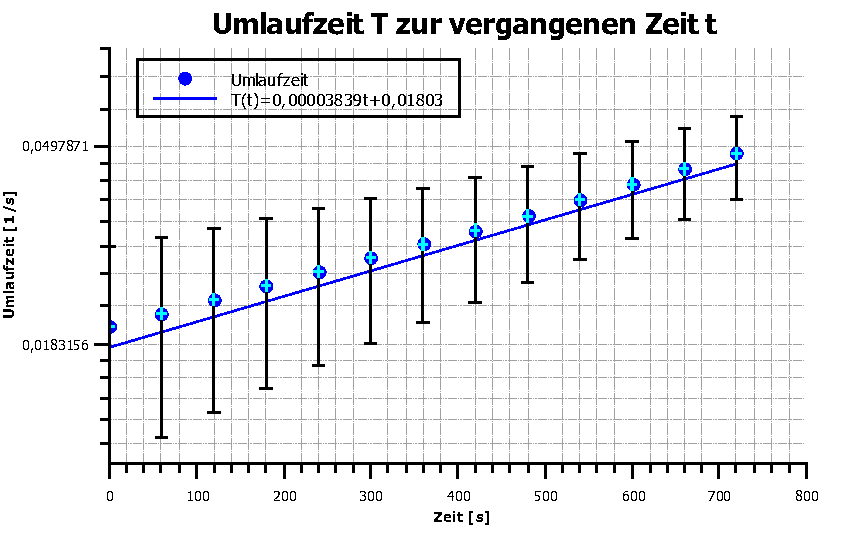
\includegraphics[width=1\textwidth]{T_gegen_t.pdf}
\caption{\label{fig:T_gegen_t}Anzugeben ist hier noch ein Fehler von etwa 0,01Hz da das Messgerät nur auf zwei Nachkommastellen angegeben hat (schwarzer Fehlerbalken). Des weiteren sollte man beachten, dass die Stoppuhr von einem Menschen betätigt wurde und die Reaktionszeit (nach Wikipedia), bei etwa 100ms liegt (hellblauer Fehlerbalken).}
\end{figure}
   
   Die logarithmische Einteilung ist in so fern sinnvoll, da sich für exponentielle Abläufe an dieser Stelle eine Gerade ergeben sollte. Schaut man sich den Abfall der Frequenzwerte an, so unterstützen diese die Aussage, dass es sich hier um einen exponentiell abfallenden Prozess handelt. Da es hier allerdings schnell zu abweichenden Messwerten kommen kann, aufgrund verschiedener Reaktionszeiten oder dem ganz genauen Ablesen des Frequenzmessgerätes, ist die Gerade nur mit einem $R^2=0,9783$ an zu geben. Im Allgemeinen spiegelt diese aber eine richtige Deutung der Messwerte.\\
	
	Um nun die Dämpfung zu berechnen hilft einem der Zusammenhang zwischen Winkelgeschwindigkeit $\omega$ und der Zeit $t$. $\omega$  berechnet sich wie folgt:
	
	$$	\omega=\frac{2\pi}{T}=2\pi \cdot f$$
	

	 
	Für die Dämpfung $\beta$ ergibt sich untenstehender Zusammenhang, mit $\omega_0$ als Anfangs-Winkelgeschwindigkeit, $t$ der Zeit und der omentanbetrachteten Wingelgeschwindigkeit $\omega(t)$:\\
	 
	 $$ \omega(t)=\omega_0 \cdot \exp(-\beta t) $$
	 $$\Rightarrow ln\omega(t)=ln\omega_0-ln(exp(-\beta\cdot t))$$
	 $$ \Rightarrow ln\omega(t) = ln\omega_0 -\beta \cdot t $$

     \begin{figure}[H]
     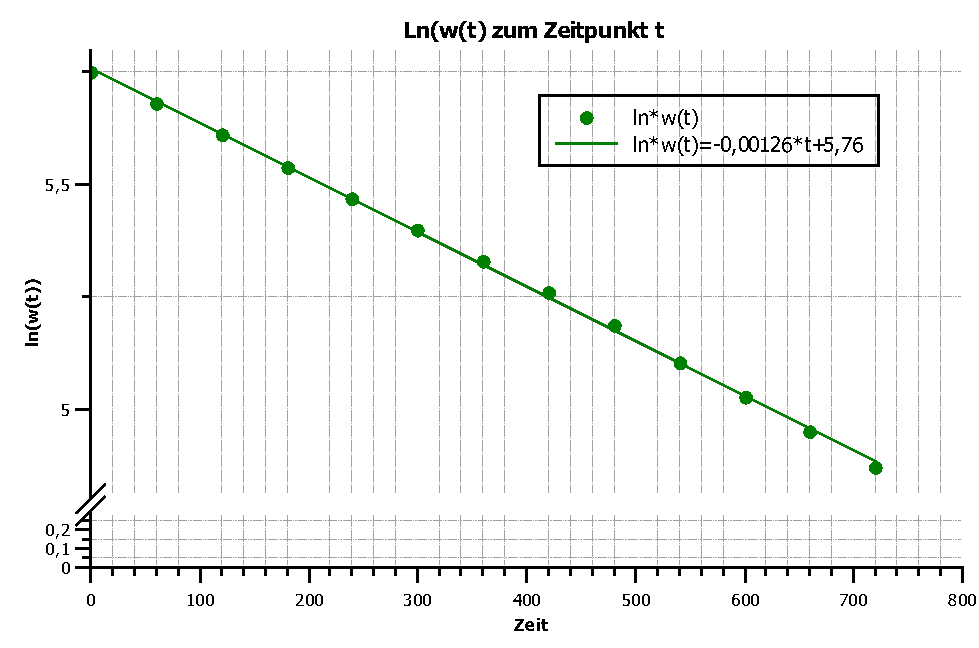
\includegraphics[width=1\textwidth]{ln_w_t__.pdf}
\caption{\label{fig:ln_w_t_}Trägt man die berechneten Werte von $ln\omega(t)$ gegen die Zeit auf, ergibt sich eine Gerade, welche die Steigung $-0,001216$ besitzt. Sie bildet unseren gesuchten Dämpfungsfaktor $-\beta$}
\end{figure}
	 
	 Um dies auch nochmal an einer Rechnung zu belegen, kann man die obige Formel noch ein bisschen weiter umformen:
	 $$\Rightarrow ln\omega(t)-ln\omega_0=-\beta\cdot t$$
	 $$\Rightarrow \beta=-\frac{ln(\frac{\omega(t)}{\omega_0})}{t}$$
	 und durch Einsetzten des ersten Messwertes ergibt sich z.\,B.:
	 $$\Rightarrow \beta=-\frac{ln(\frac{299,55}{314,159})}{60}=0,00113$$
Wie man also sieht stimmt die Rechnung mit
 der Steigung überein.

\end{document}